\section{氧气的制法}\label{sec:1-3}

在实验室里,一般用给氯酸钾或高锰酸钾加热的方法来制取氧气。
用氯酸钾制取氧气,通常还要放入少二氧化锰\footnote{或者放入少量氧化铁等。},
这是为什么呢?让我们仔细观察下面三个实验。

\begin{shiyan}
    把少量氯酸钾放在试管里加热几分钟,可以看到,氯酸钾熔化后,才开始缓慢地放出气泡,
    这时用带火星的木条插入管口,观察木条是否着火。如果着火,表明有什么气体放出?
\end{shiyan}

\begin{shiyan}
    把少量二氧化锰放在试管里加热,用带火星的木条插入管口,观察木条是否着火。
    这种现象表明有没有氧气放出?
\end{shiyan}

\begin{shiyan}
    把少量氯酸钾放在试管里稍稍加热片刻,即用带火星的木条插入管口,木条不着火。
    把试管移离火焰,迅速撒入少量二氧化锰,再用带火星的木条插入管口,观察木条是否着火。
    这个实验说明什么问题?
\end{shiyan}


从上面的实验可以看到,给氯酸钾加热到较高温度时,有氧气放出,给二氧化锰加热,并没有氧气放出,
只有往氯酸钾里加入二氧化锰,不需加热到高温就有氧气放出。
这几个实验说明,受热不放出氧气的二氧化锰,却有使氯酸钾在较低的温度下迅速放出氧气的作用。
人们还通过实验证明,二氧化锰在这个反应里并没有消耗,反应前加入多少,反应后仍有多少,并且化学性质没有改变。
这种\zhongdian{在化学反应里能改变其它物质的化学反应速度,而本身的质量和化学性质在化学反应前后都没有改变的物质,叫做催化剂(或触媒)。}
催化剂在反应里所起的作用叫做\zhongdian{催化作用}。二氧化锰是这个反应的催化剂,它在这个反应里起催化作用。
在许多化学工业里,如生产硫酸、合成氨都要采用适当的催化剂来加快化学反应速度,以提高单位时间的产量。

给氯酸钾加热,除生成氧气外,还生成另一种物质氯化钾。这个化学反应可以表示如下:
\begin{fangchengshi}
    \ce{ \text{氯酸钾} ->[\text{催化剂}][\text{加热}] \text{氯化钾} + \text{氧气} }
\end{fangchengshi}

氧气不易溶于水,可用排水法收集(图\ref{fig:1-9})。

\begin{figure}[htbp]
    \centering
    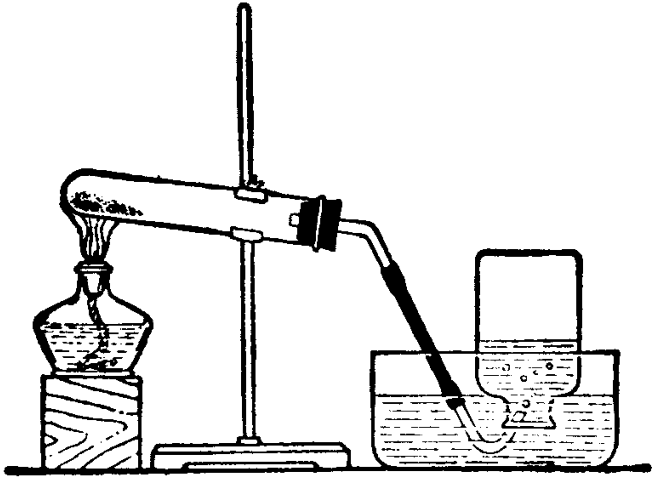
\includegraphics[width=9cm]{../pic/czhx1-ch1-9}
    \caption{制取氧气}\label{fig:1-9}
\end{figure}

\begin{shiyan}
把氯酸钾和二氧化锰混和(一般按 $3:1$ 的质量比混和)均匀后,放在试管里,用带有导管的塞子紧塞管口。
给试管加热。用排水法收集氧气一瓶。怎样用简单的方法证明集气瓶里收集的是氧气。
\end{shiyan}

高锰酸钾比氯酸钾容易分解,只要稍稍加热就能放出氧气,不需用催化剂。
给高锰酸钾加热生成氧气的化学反应,可以表示如下:
\begin{fangchengshi}
    \ce{ \text{高锰酸钾} ->[\text{加热}] \text{锰酸钾} + \text{二氧化锰} + \text{氧气} }
\end{fangchengshi}

在给氯酸钾加热制氧气的反应里,氯酸钾生成了氯化钾和氧气。
在给高锰酸钾加热制氧气的反应里,高锰酸钾生成了锰酸钾、二氧化锰和氧气。
这类\zhongdian{由一种物质生成两种或两种以上其它物质的反应,叫做分解反应。}

工业上用的大量氧气,主要是用分离空气的方法制取的。
例如,在低温下加压,把空气转变为淡蓝色的液态空气,然后蒸发。
由于液态氮的沸点($-196$ ℃)比液态氧的沸点($-183$ ℃)低,氮气先从液态空气里蒸发出来,剩下的主要就是液态氧了。
为了便于贮存、运输和使用,通常给氧气加到 $150$ 标准大气压,贮存在氧气瓶里。

\begin{xiti}

\xiaoti{实验室用氯酸钾制取氧气和工业上用空气制取氧气,在哪种方法里发生物理变化,哪种方法里发生化学变化?为什么?}

\xiaoti{实验室用氯酸钾制取氧气时,为什么要加二氧化锰?为什么可以用排水法收集氧气?}

\xiaoti{用文字完整地表示下列化学反应,并指明其中哪些属于分解反应,哪些属于化合反应。}
\begin{xiaoxiaotis}

    \xxt{\ce{ \text{磷} + \text{\ewkh[3em]} ->[\text{点燃}] \text{五氧化二磷} }}

    \xxt{\ce{ \text{铝} + \text{\ewkh[3em]} ->[\text{加热}] \text{三氧化二铝} }}

    \xxt{\ce{ \text{高锰酸钾} ->[\text{加热}] \text{氧气} + \text{\ewkh[3em]} + \text{\ewkh[3em]} }}

    \xxt{\ce{ \text{氯酸钾} ->[\text{催化剂}][\text{加热}] \text{氧气} + \text{\ewkh[3em]} }}

\end{xiaoxiaotis}

\end{xiti}


